% ==================== 2.3.2.7 萤石 ====================
\jiegou{2.3.2.7}{萤石结构（\texorpdfstring{CaF$_2$}{CaF2}）}

以 CaF$_2$ 为例建立模型，建模参数见表~\ref{tab:fluorite}。萤石结构中 Ca$^{2+}$ 占据
面心立方位置，F$^-$ 占据晶胞内全部 8 个四面体间隙。

\begin{table}[H]
  \centering
  \caption{萤石（CaF$_2$）结构的建模参数}
  \label{tab:fluorite}
  \begin{tabular}{ll}
    \toprule
    项目 & 参数 \\
    \midrule
    空间群 & $F\,m\,\bar3\,m$（No.~225） \\
    晶格常数 & $a=b=c=5.462$\,\AA，$\alpha=\beta=\gamma=90^\circ$ \\
    原子坐标 & Ca：$(0,0,0)$（$4a$ 位）；F：$(1/4,1/4,1/4)$（$8c$ 位） \\
    化学式单元数 & $Z=4$ \\
    \bottomrule
  \end{tabular}
\end{table}

\begin{figure}[H]
  \centering
  \subcaptionbox{(a) 空间群与晶格常数设置}{%
    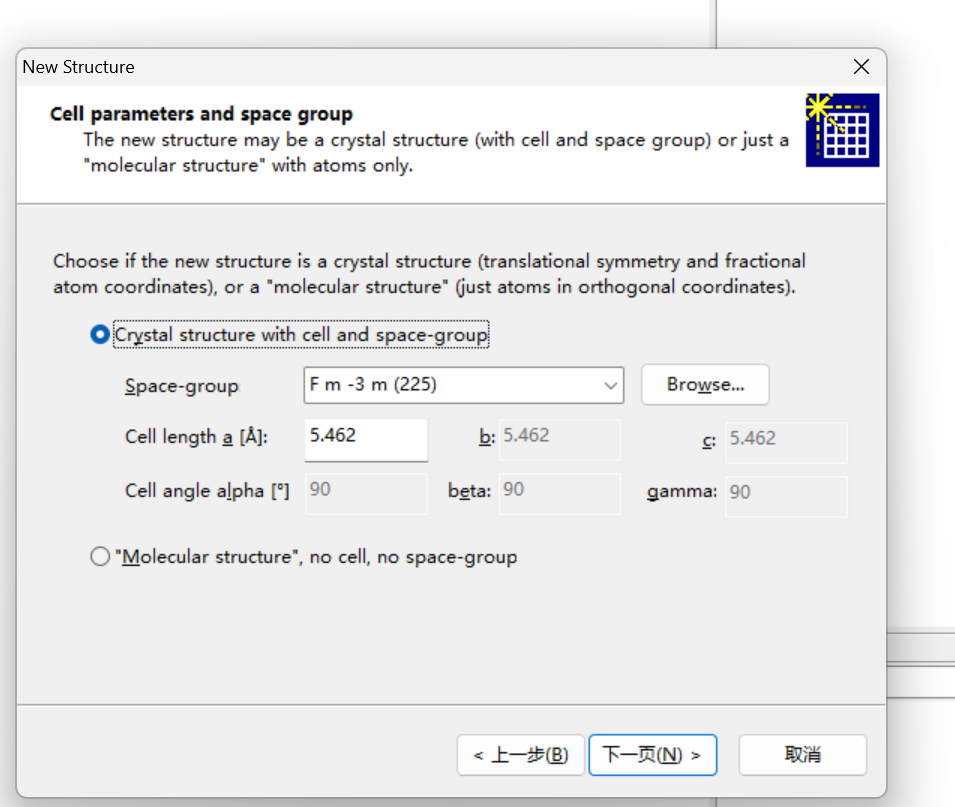
\includegraphics[width=0.44\textwidth]{assets/fluorite/a.png}}
  \hfill
  \subcaptionbox{(b) 非对称单元原子（Ca、F）添加}{%
    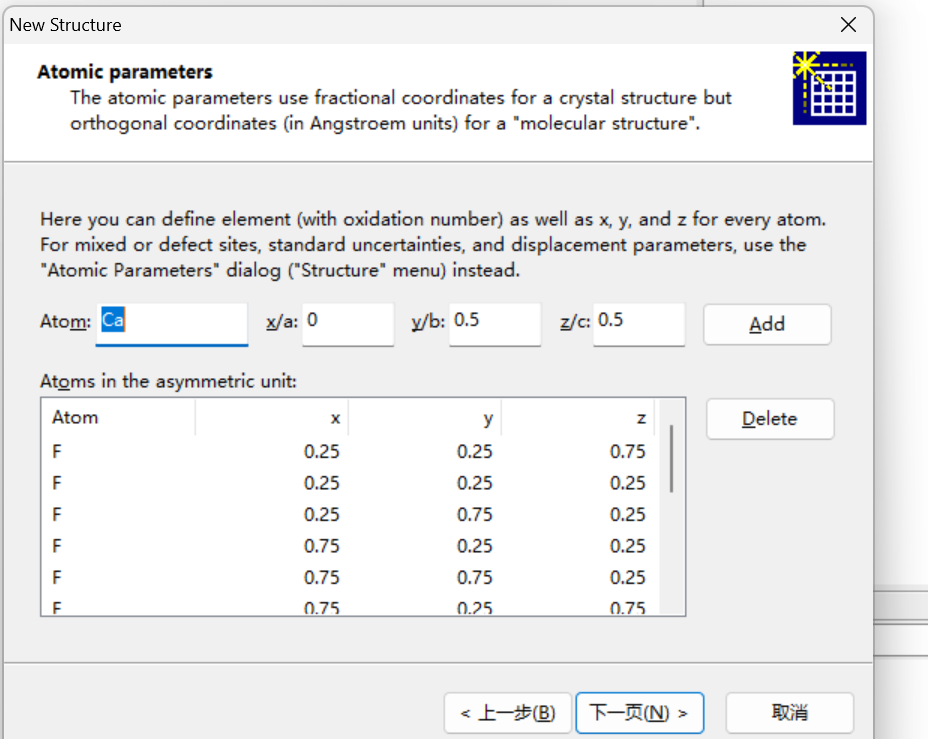
\includegraphics[width=0.44\textwidth]{assets/fluorite/b.png}}
  \caption{萤石（CaF$_2$）结构的参数设置}
  \label{fig:fluorite-param}
\end{figure}

\begin{figure}[H]
  \centering
  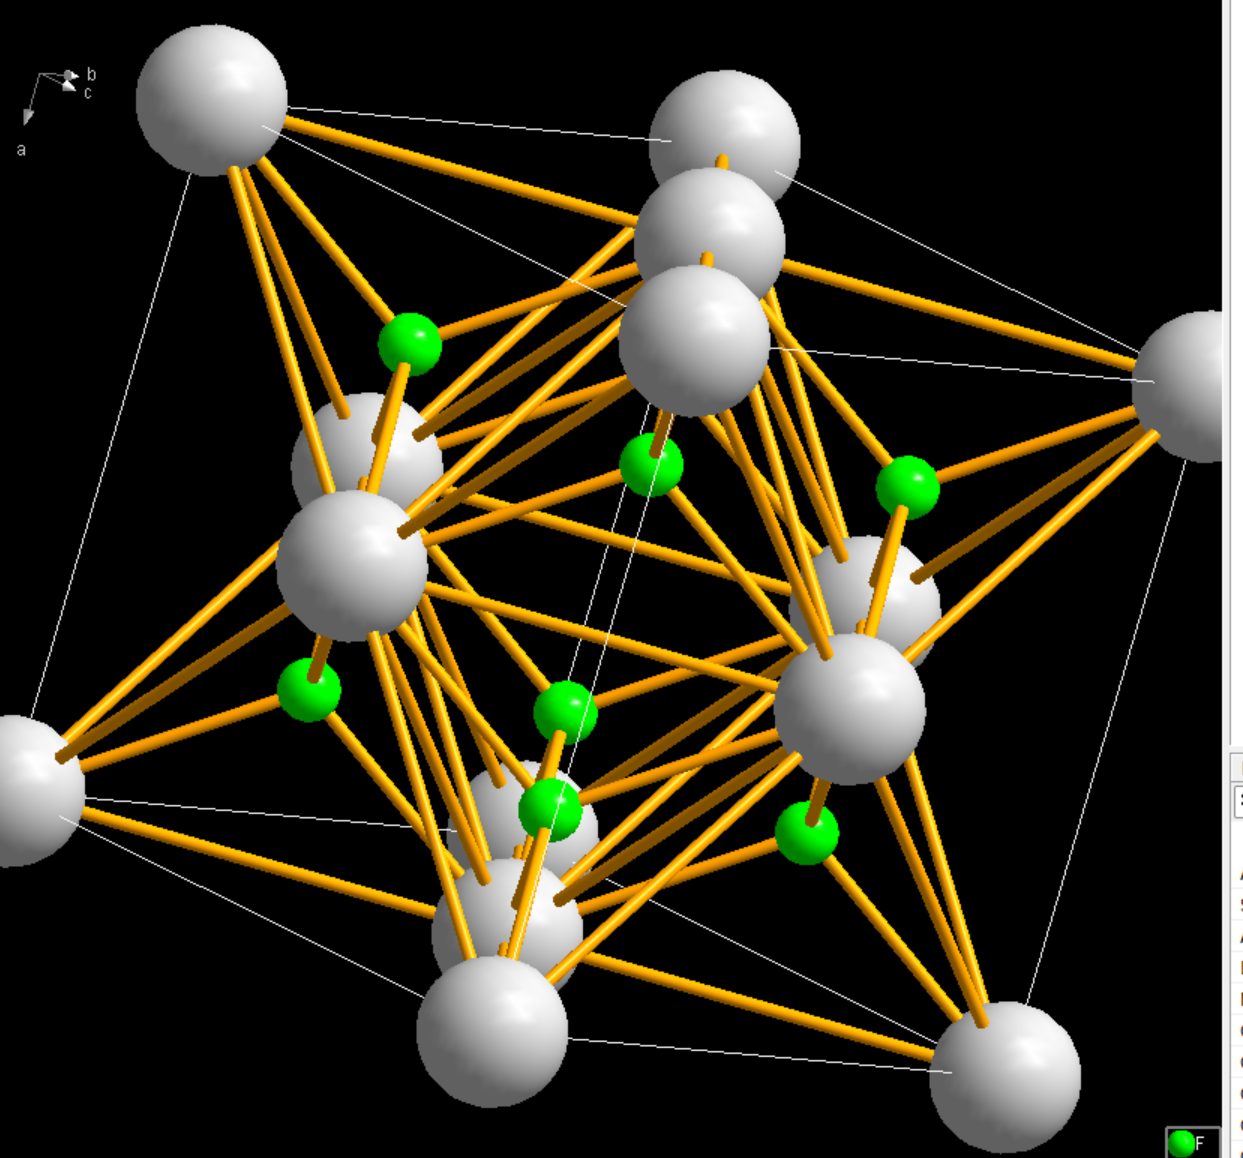
\includegraphics[width=0.5\textwidth]{assets/fluorite/c.png}
  \caption{萤石（CaF$_2$）结构的晶体结构模型}
  \label{fig:fluorite-model}
\end{figure}

\begin{figure}[H]
  \centering
  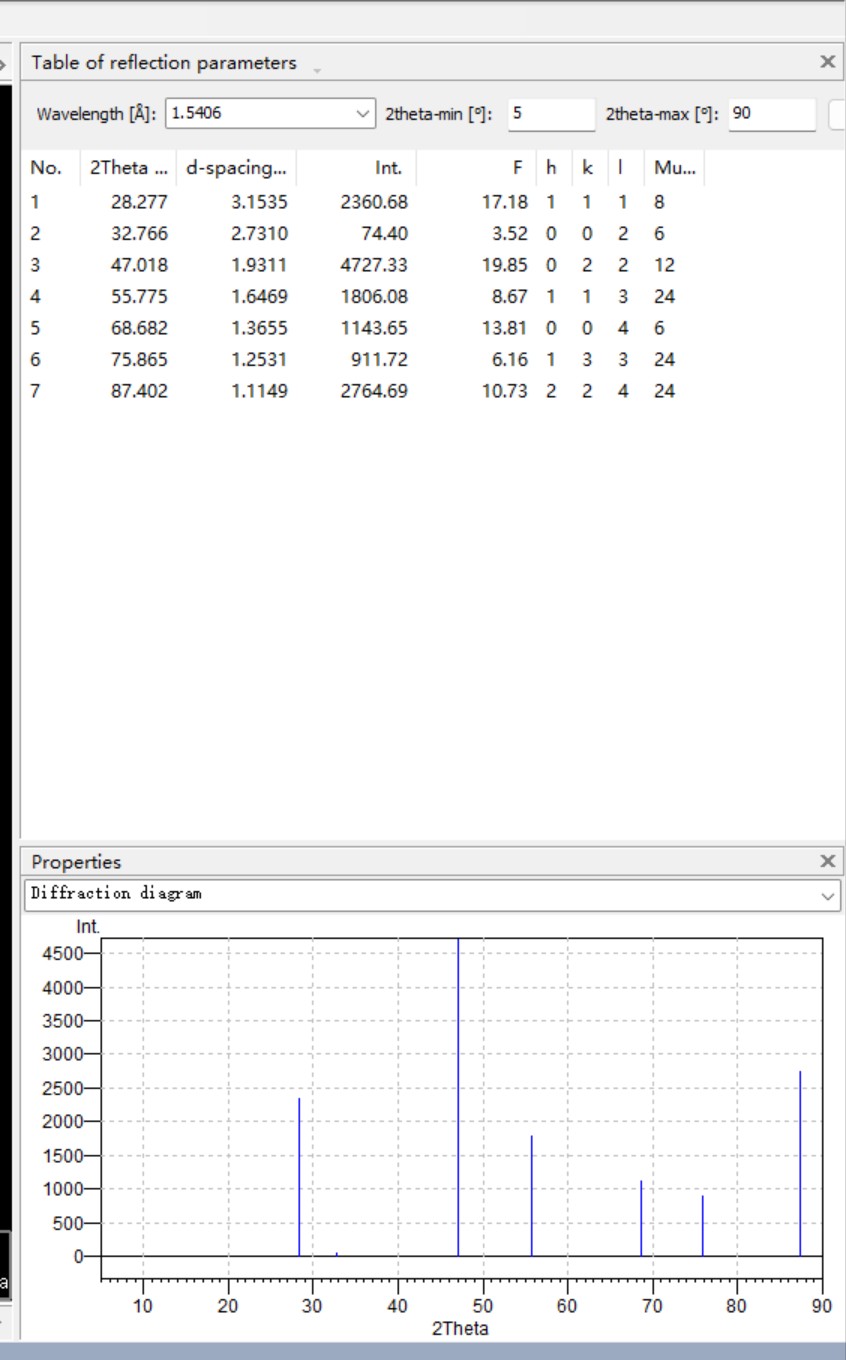
\includegraphics[width=0.4\textwidth]{assets/fluorite/d.png}
  \caption{Diamond 模拟的萤石（CaF$_2$）结构粉末衍射图}
  \label{fig:fluorite-xrd}
\end{figure}

\begin{figure}[H]
  \centering
  \subcaptionbox{(a) 晶面视图}{%
    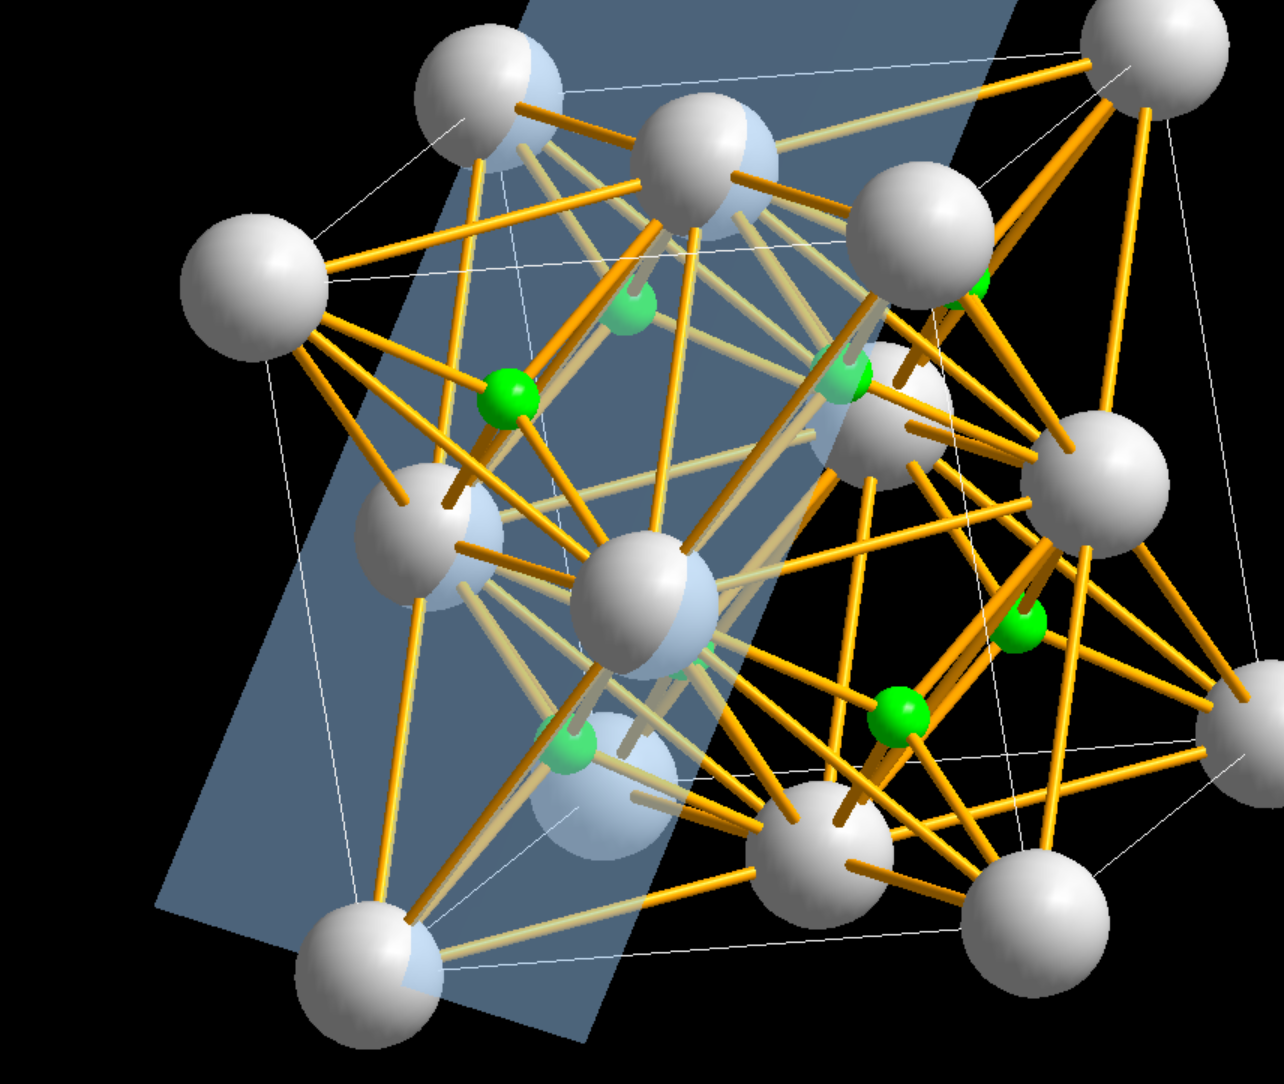
\includegraphics[width=0.44\textwidth]{assets/fluorite/e.png}}
  \hfill
  \subcaptionbox{(b) Ca 的立方配位与 F 的四面体配位}{%
    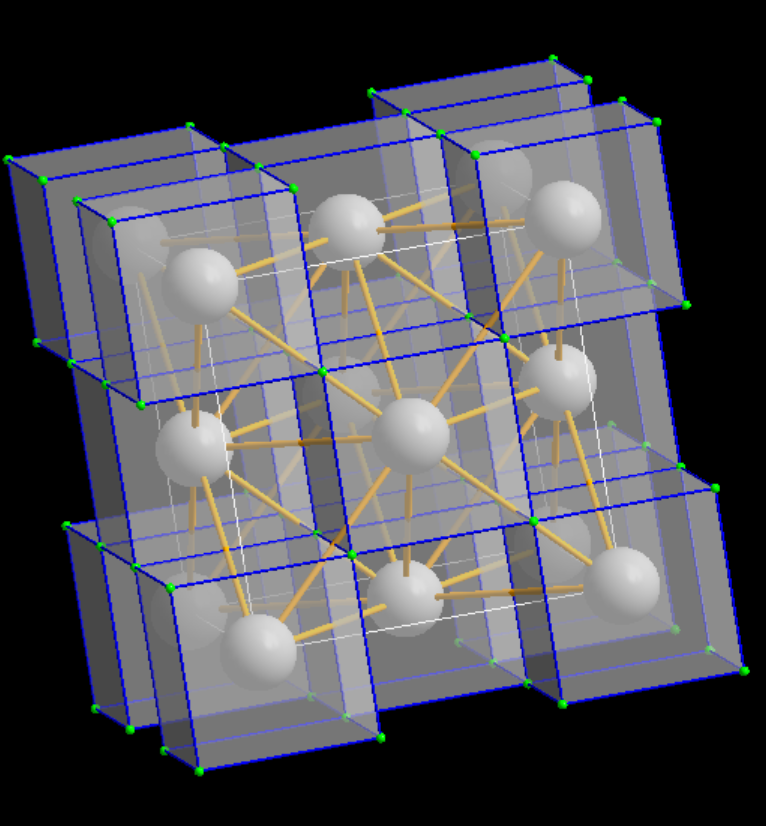
\includegraphics[width=0.28\textwidth]{assets/fluorite/f.png}}
  \hfill
  \subcaptionbox{(c) 配位多面体设置}{%
    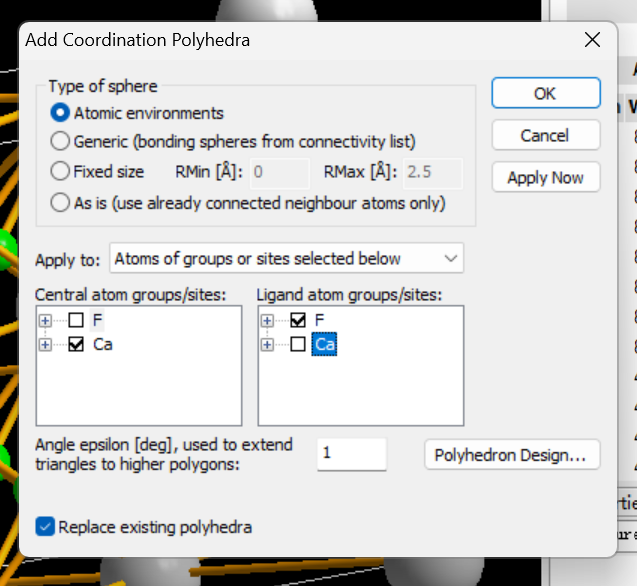
\includegraphics[width=0.24\textwidth]{assets/fluorite/f1.png}}
  \caption{萤石（CaF$_2$）结构的晶面与配位多面体}
  \label{fig:fluorite-plane}
\end{figure}

\textbf{结构特征。}萤石结构可用两种视角描述：Ca$^{2+}$ 构成面心立方骨架，F$^-$ 填充
其中全部 8 个四面体间隙；或视为 F$^-$ 构成简单立方骨架，Ca$^{2+}$ 间隔填充其中一半
立方体空隙。

\begin{enumerate}[label=（\arabic*）]
  \item \textbf{配位数}：Ca$^{2+}$ 被 8 个 F$^-$ 包围，配位多面体为立方体
    （图~\ref{fig:fluorite-plane}(b)）；F$^-$ 被 4 个 Ca$^{2+}$ 包围，配位多面体为
    四面体。键长 $d=\sqrt{3}a/4=\sqrt{3}\times5.462/4\approx2.37$\,\AA。
  \item \textbf{间隙填充}：面心立方点阵的四面体间隙（如 $(1/4,1/4,1/4)$ 及其对称
    等效位置）共有 8 个，在萤石结构中被 F$^-$ 全部占据，而八面体间隙
    $(1/2,1/2,1/2)$ 保持空缺。这种``部分填充''特点使萤石结构具有较高的离子迁移空间，
    ZrO$_2$、CeO$_2$ 等萤石型氧化物是重要的快离子导体与燃料电池电解质材料。
  \item \textbf{反萤石结构}：若阴阳离子互换（碱金属占据 F$^-$ 位、O$^{2-}$ 占据
    Ca$^{2+}$ 位），即得反萤石结构，如 Na$_2$O、Li$_2$O。
\end{enumerate}

具有萤石型结构的典型物质包括 CaF$_2$、BaF$_2$、UO$_2$、ThO$_2$ 及高温相 ZrO$_2$ 等。
